\documentclass[11pt]{article}
\usepackage{amsmath, amsfonts, amsthm, amssymb}
\usepackage{float}
\author{Methum Kasthuriarachchi}
\title{Buffon Needles and Noodles}

\usepackage{graphicx}

\begin{document}
\maketitle

\section{Introduction}
For this project, I wrote Matlab code to simulate the Buffon's Needle problem and its variant, Buffon's Noodle. 

\section{Buffon's Needles and Noodles Code}
For all cases of the simulation, the grid was set up to be from 0 to 5 for both the x and y axis. The entire length of the needle/noodle for all simulations was 1.

\subsection{Simulating dropping straight needles}
The function straight\underline{\hspace{0.2cm}}needle\underline{\hspace{0.2cm}}drop, shown in figure \ref{fig:C1}, generates the needles that will be animated in later as the points are connected. To create the points, I randomly picked the middle of the line to be from 0.5 to 4.5. I did this because I wanted to make sure that the line would still be able to hit the horizontal axis if it's midpoint happened to be at the lowest or possible y values.

\begin{figure}[H]
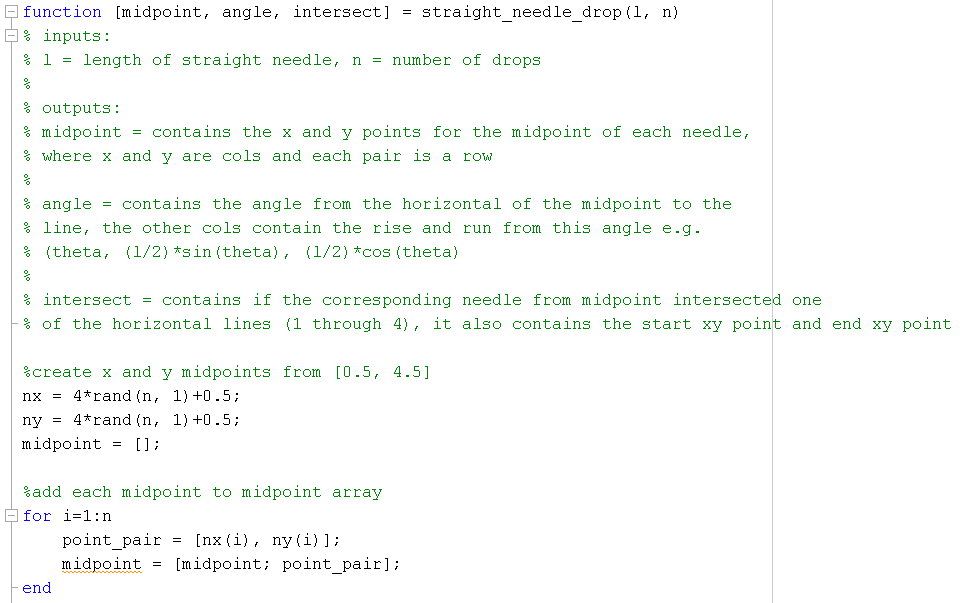
\includegraphics[width=\textwidth, height = 2.2in]{f1.png}
\caption{Create midpoints for straight needles}
\label{fig:C1}
\end{figure}

 I would then generate an angle to orient the line. Through this angle, and because the lenght of the line is know, I can generate the x and y endpoints for each line. These endpoints are stored in the array intersect. I then check to see if the lines are intersected based on the middle point. A variable that contains whether the line was intersected is also stored in the intersect array. This can be seen in figure \ref{fig:C2}.

\begin{figure}[H]
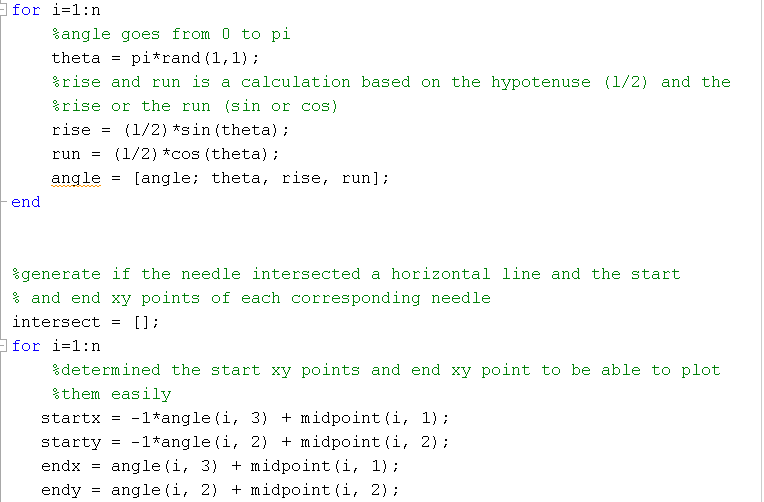
\includegraphics[width=\textwidth, height = 2.2in]{f2.png}
\caption{Find rise and run through the angles, then determine x and y position through the midpoint.}
\label{fig:C2}
\end{figure}

After that, I can determine the intersection points of the lines by checking the midpoint and the endpoints, as seen in figure \ref{fig:C3} for each of the horizontal lines (y = 1, 2, 3, and 4).

\begin{figure}[H]
\begin{centering}
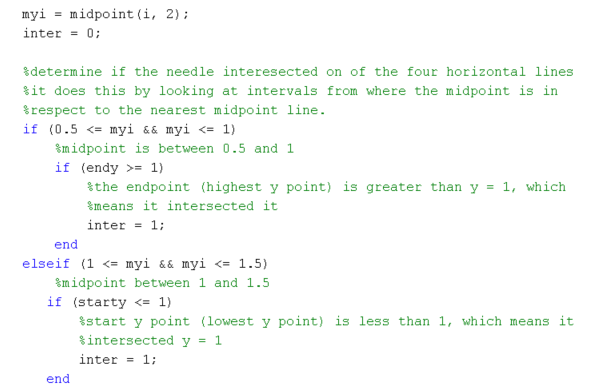
\includegraphics[width=\textwidth, height = 2in]{f3.png}
\end{centering}
\caption{Find rise and run through the angles, then determine x and y position through the midpoint.}
\label{fig:C3}
\end{figure}

Both start and end point's x and y values, as well as if the line intersected is then stored in the intersect array, as show in figure \ref{fig:C4}. 

\begin{figure}[H]
\begin{centering}
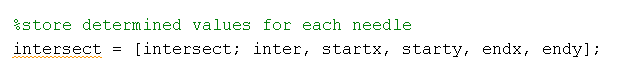
\includegraphics[scale=.7]{f4.png}
\end{centering}
\caption{Find rise and run through the angles, then determine x and y position through the midpoint.}
\label{fig:C4}
\end{figure}

These points can then be combined using the plot command in Matlab to create the needles, seen in figure \ref{fig:d1}. I decided to make the needles blue if they intersected the red horizontal lines, and black if they didn't intersect.

\begin{figure}[H]
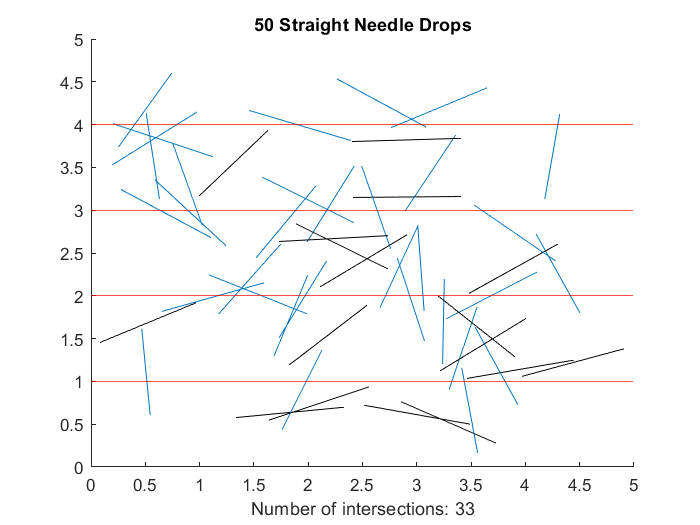
\includegraphics[width=0.6\textwidth]{straight.png}
\caption{Dropping 50 straight needles. Blue needles means they intersected; black lines means no intersection.}
\end{figure}
\label{fig:d1}
%end 

\subsection{Simulating dropping needles bent once}
The function bent\underline{\hspace{0.2cm}}needle\underline{\hspace{0.2cm}}drop, shown in figure \ref{fig:C5}, generates a needle bent once. This can both create needles with an angle between the legs to be a constant chosen by the user, or a random angle from $\frac{\pi}{6}$ to $\frac{5\pi}{6}$, as seen in \ref{fig:d2} which contains the bent needle with a constant angle and \ref{fig:d3} which shows the bent needle with an inbetween angle that is random. To create these needles I first started out by choosing the midpoints, which is the same as what I did in figure \ref{fig:C1}. 

\begin{figure}[H]
\begin{centering}
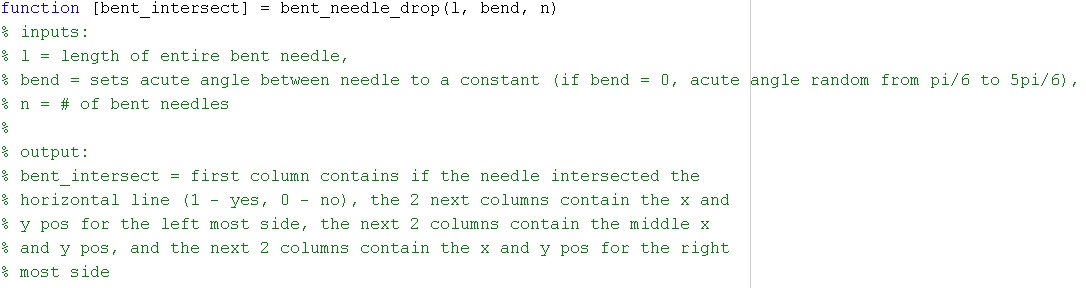
\includegraphics[scale=0.5]{f5.png}
\end{centering}
\caption{The function that drops the bent needles. In the comments includes the inputs, and the outputs of the function.}
\label{fig:C5}
\end{figure}

\begin{figure}[H]
\begin{centering}
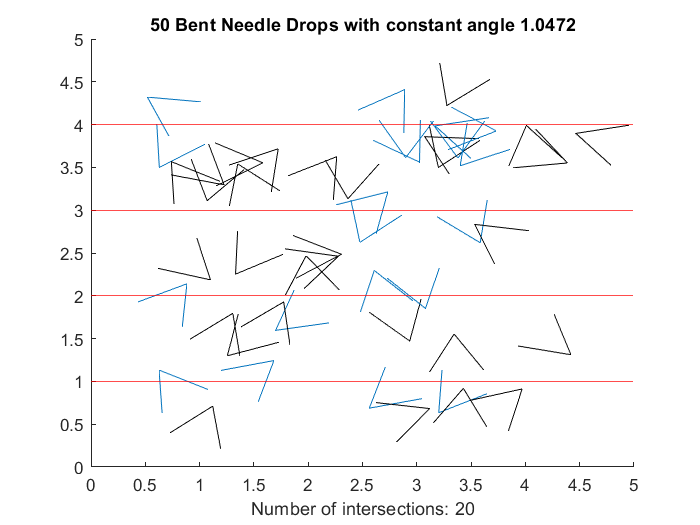
\includegraphics[width=0.6\textwidth]{bent_constant.png}
\end{centering}
\caption{Dropping bent needle with an inbetween angle that is constant.}
\label{fig:d2}
\end{figure}

\begin{figure}[H]
\begin{centering}
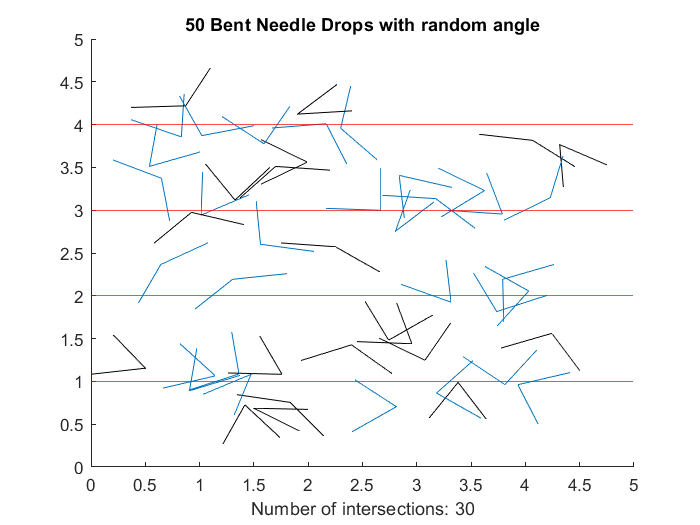
\includegraphics[width=0.6\textwidth]{bent_random.png}
\end{centering}
\caption{Dropping bent needle with an inbetween angle that is random.}
\label{fig:d3}
\end{figure}

After generating the midpoint (the vertex) of the needle, I needed to create two other points. To do this I generated two angles, one to orient it as if there was a line through the middle, similar to figure \ref{fig:C2}, but also another angle that determines the random inbetween angle, as seen in figure \ref{fig:C6}.
\begin{figure}[H]
\begin{centering}
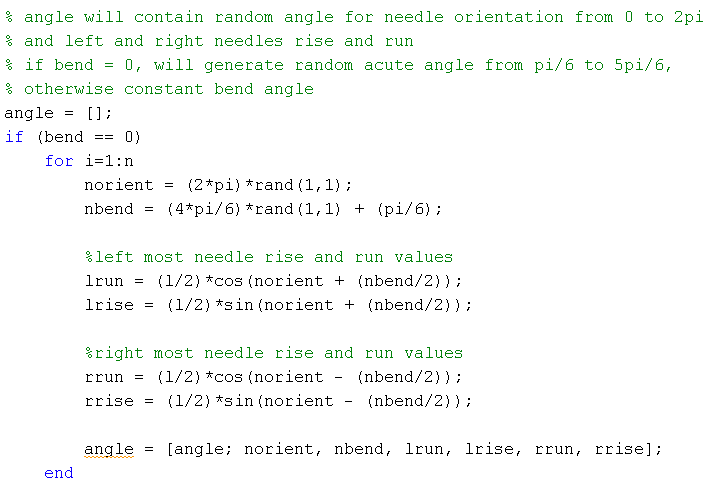
\includegraphics[scale=0.5]{f6.png}
\end{centering}
\caption{Generate random angles and rise and run based on it for the two other points for the bent needle.}
\label{fig:C6}
\end{figure}

After that I can determine the points for those two lines, and whether they intersect as seen in figure \ref{fig:C7}.
\begin{figure}[H]
\begin{centering}
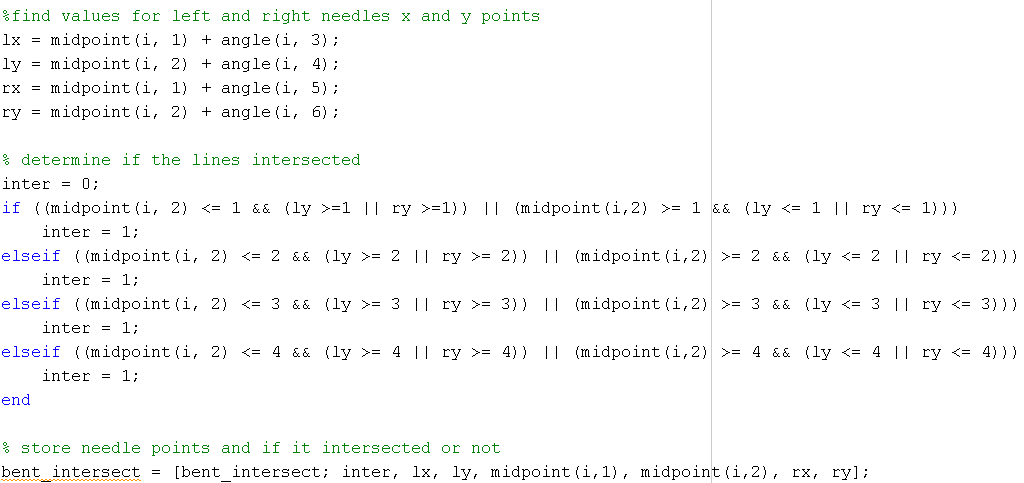
\includegraphics[scale=0.5]{f7.png}
\end{centering}
\caption{Determine the x and y points for the other two points to create a bent needle, and determine whether it intersects one of the horizontal lines or not. Then store those values to be used in array bent\underline{\hspace{0.2cm}}intersect.}
\label{fig:C7}
\end{figure}

%end 

\subsection{Simulating dropping needles bent twice}
The function drop\underline{\hspace{0.2cm}}noodle, generates the points and drops needles bent twice randomly and counts the number of intersections, but also if the intersection is positive or negative based on the preferred end (seen in figure \ref{fig:d4}). 

\begin{figure}[H]
\begin{centering}
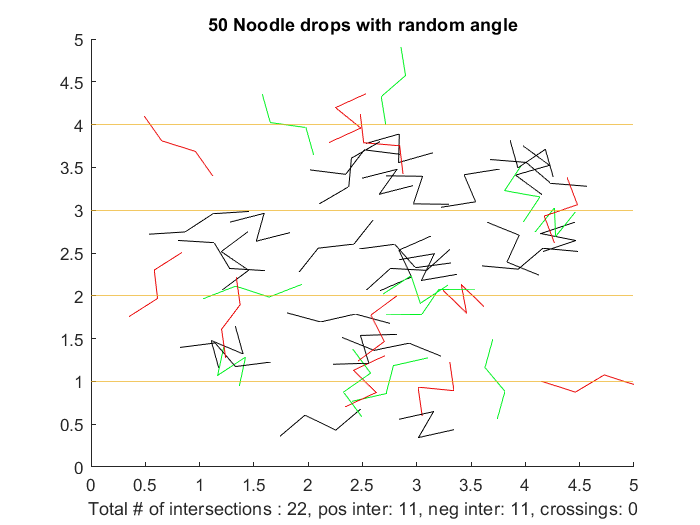
\includegraphics[width=0.6\textwidth]{noodle.png}
\end{centering}
\caption{Drop 50 random noodles. Green noodles account for the positive intersections, red noodles count for the negative intersections, blue intersections are meant to count when the preferred end lands on a horizontal line exactly, and black lines represent no intersections. The crossing values is created by summing the positive and negative intersections.}
\label{fig:d4}
\end{figure}

To create this, I started out using the same methods to make the bent noodle, seen in section 2.2. To create the third line I had to determine the angle based on the orientation and in between angle, as seen in figure \ref{fig:C8}.
\begin{figure}[H]
\begin{centering}
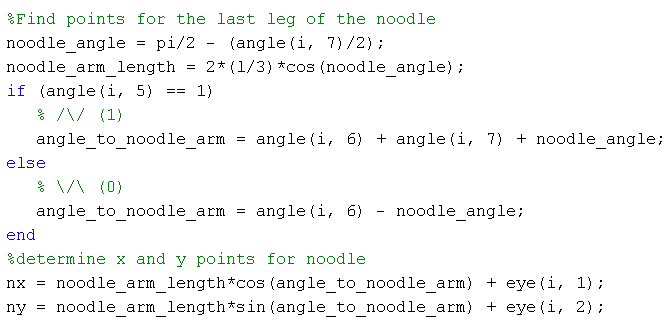
\includegraphics[scale=0.5]{f8.png}
\end{centering}
\caption{Determine the x and y points for the third line that will be connected to the bent needle.}
\label{fig:C8}
\end{figure}

I then have to check for the intersection based on the end points of the noodle and whether there is a positive or negative intersection based on the preferred end, as seen in figure \ref{fig:C9}.
\begin{figure}[H]
\begin{centering}
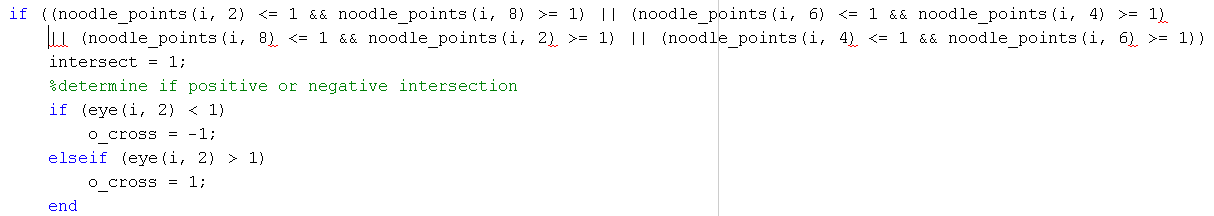
\includegraphics[scale=0.5]{f9.png}
\end{centering}
\caption{Determine if the endpoints of the noodle intersected any of the horizontal lines, and then check if the intersection is positive or negative.}
\label{fig:C9}
\end{figure}
%end 

\subsection{Conjecture for average crossing number for needles bent twice}
The average crossing number for the noodles (Number of positive intersections - Number of negative intersections) should be 0. Given that a random amount of noodles intersect certain horizontal lines. Because the intersections are random, there should be roughly half that have the preferred end over the top of the line and half that are under the line. Giving us an equal number of positive and negative intersections, meaning that the average crossings for the noodles should equal 0, which can be seen in figure \ref{fig:d4}.

%end 
\end{document}
